\documentclass[letterpaper, conference]{IEEEtran}  % Comment this line out if you need a4paper
\setlength  {\textheight}    {9.2in}
\setlength  {\textwidth}     {6.8in}
%\setlength  {\oddsidemargin} {0.1in}
%\setlength  {\evensidemargin}{0.1in}
%\setlength  {\voffset}{-0.6in}
\parindent 0pt 
\parskip 1ex 
\setlength{\unitlength}{1in} 

\usepackage{hyperref}
\setlength{\unitlength}{1in} 
\usepackage{amsmath, amsfonts, amssymb, amscd} 
\usepackage[usenames,dvipsnames]{color} 
\usepackage[capitalize]{cleveref}
\usepackage{longtable}
\usepackage{pdfpages}
\usepackage{pgfplots}
\usepackage{nomencl}
\usepackage{subcaption}


\makenomenclature
\usepackage[per-mode=symbol,mode=text,group-separator={,},group-four-digits=true,load=accepted,list-final-separator={, and }]{siunitx}
%\usepackage[section]{placeins}

\newunit{\hour}{hours}
\newunit{\feet}{ft}
\newunit{\nauticalmile}{NM}
\newunit{\gravity}{g}
\newunit{\mph}{mph}
\newunit{\knots}{knots}
\hypersetup{
    colorlinks=true,
    hypertexnames=false,
    plainpages = false,
    breaklinks=true,
    a4paper=false,
    linkcolor = black,  % Non printing boxes
    anchorcolor = black,
    citecolor = black,
    filecolor = black,
    menucolor = black,
    urlcolor = blue,
    pdfauthor={Zouhair Mahboubi},
    pdftitle={CS231A Project Proposal}
}

\usepackage{fancyhdr} 
\pagestyle{fancy}
\fancyhf{}
\renewcommand{\headrulewidth}{0.5pt}
\fancyfoot[c]{\footnotesize{CS231A Project Final Report}}
\fancyfoot[l]{\footnotesize{}}
\fancyfoot[r]{\footnotesize\sffamily\thepage}
\fancypagestyle{plain}{
\renewcommand{\headrulewidth}{0pt}
}

\usepackage[backend=bibtex]{biblatex}
\addbibresource{Research.bib}


\title{Above Ground Altitude Estimation for General Aviation Aircraft During Landing Phase\\
\vspace{1cm}
\small{CS231A Project Report}}
\author{Zouhair Mahboubi} 
\begin{document} 
\maketitle 
%\tableofcontents 
% \listoffigures 
%\newpage 


%

%6 Sections:



%Sec 4: Experiments — present your experimental results of the method you have implemented with plots, graphs, images and visualizations. Show numerical/quantitative and qualitative results. Show a performance analysis on the mobile device in term of efficiency, speed, memory and computational demands.
%Sec 5: Conclusions — what's the take home message?


%%%%%%%%%%%%%%%%%%%%%%%%%%%%%%%%%%%%%%%%%%%%%%%%%%%%%%%%%%%%%%%%%%%%%%%%%%%%%%%%
%Abstract: A short summary of the project with main results.
\begin{abstract}
Accurately judging the above-ground altitude (AGL) is an important skill to safely land an airplane. Pilots rely on visual cues to determine their AGL, but it takes many hours for a student pilot to hone this skill. In this project, we explore the use of an on-board camera to provide AGL as a helping tool that could be used as part of training new pilots. We collected data from a cockpit view of an aircraft, and implemented a pipeline which detects runway edges and estimates the aircraft AGL. Final results were noisy and could benefit from Kalman filtering.
\end{abstract}

%Sec 1: Introduction: introduce the problem you want to solve, explain why it is important to solve it.
\section{Introduction}
Ask a student pilot what the most difficult part of flying is, and you will often get landing as an answer (Air Traffic Control comes in as a close second). Indeed, landings account for more than a third of all general aviation (GA) accidents. While they are often non-fatal due to the relatively low energies involved, they are responsible for hundreds of damaged aircraft per year \cite{Aviat2012}.

Aircraft (most of them at least) are designed to fly: Line one down the runway and throttle up, and it will pick up enough speed and take-off. In an introductory flight lesson, after a one hour ground lesson (including some simulator time), a student pilot will be able to take-off with minimal supervision. Landing on the other hand is a "controlled crash", where the aircraft is brought to its slowest possible flying speed and stalled a few feet near the ground. This is known as the Roundout or the Flare, and it often takes tens of hours and hundreds of landings before the student masters the art of landing and can fly solo.

What makes flaring an aircraft so difficult? There has been a fair amount of research into the physiological aspect of landing, and the focus is on the use of visual cues to time the flare. This is a rather difficult skill that pilots eventually learn in order to properly judge the time to flare \cite{Palmisano2005}. Instructors and flying handbooks provide tricks and tips to help with this, but it all boils down to using the visual cues. These cues are used to estimate the height above the ground and therefore the time to contact, which in turn helps determining when the pilot needs to transition the aircraft from a descent path to a path parallel to the runway as illustrated in \cref{fig:flare}.


\begin{figure}[ht]
\centering
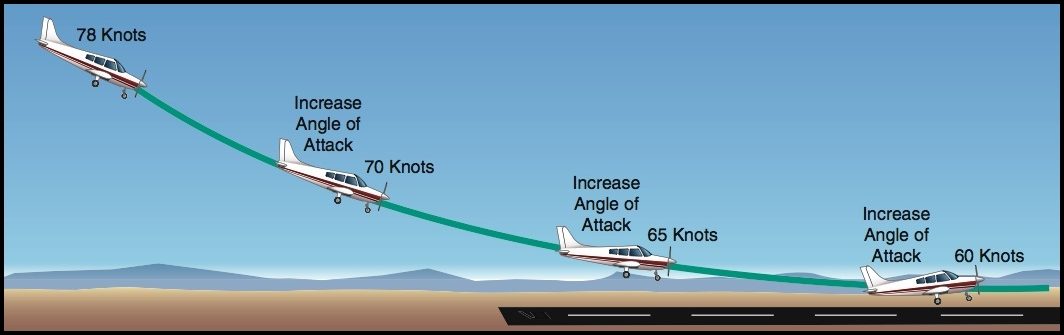
\includegraphics[width=\columnwidth]{flare.jpg} 
\caption{When the angle of attack is increased, the lift is momentarily increased, which decreases the rate of descent.  During the roundout (flare), the airspeed is being decreased to touchdown speed while the lift is being controlled so the airplane will settle gently onto the landing surface (source \cite{FAASafety}).}
\label{fig:flare}
\end{figure}

While flying, a pilot has access to a wide range of instruments to help determine the state of the aircraft (airspeed, attitude, etc.), but there rarely is one for above ground altitude (AGL). A pressure altimeter is used throughout the flight to control altitude, but its slow time constant and inaccuracy are inappropriate for the flaring task. A Global Positioning System (GPS) can provide altitude, but even with selective availability turned off, vertical accuracy is only $\SI{5}{meters} (\SI{15}{feet}$). If a Satellite Based Augmentation System (SBAS) such as Wide Area Augmentation System (WAAS) is available, this can be reduced to $\SI{1.3}{meters} (\SI{4}{feet}$) in practice. While SBAS might be accurate enough, not all GPS chipsets (especially those in mobile devices) support it, and WAAS is currently only available in North-America \cite{WAASwiki}

%Sec 2.1: Review of previous work (i.e. previous methods that have explored a similar problem).
%Sec 2.2: Describe why your method is better than previous work. Summarize the key main contributions of your work
\section{Previous Work}
The problem of accurately measuring aircraft AGL has been well studied, especially in the context of autonomous landing for aircraft which was pioneered by the British due to notoriously foggy London \cite{Autolandwiki}. Most modern civilian aircraft are equipped with radar altimeters that are used as part of autoland functionalities \cite{RadioAltskybrary}. However, radio altimeters are not used on small aircraft. This is due to weight and power constraints, and the associated costs of developing and certifying such a system. That being said, some have proposed radio altimetry to help with the task of flaring small aircraft. \citeauthor{vidmar2006} implemented a system with tonal beeps proportional to AGL \cite{vidmar2006}. FlareAssist\texttrademark \cite{FlareAssist} is a commercially available product which annunciates AGL below 15ft in 1-2 ft increments. However, it costs \$2500 and can only be used on experimental aircraft as it is not FAA certified.

An alternative way to determine the aircraft AGL is to utilize a vision system. While the use of vision for civilian autoland systems is not ideal as it is often needed when visual conditions are poor, it is an active area of research for autonomous landing of Unmanned Air Vehicles \cite{Kong2014}. There are a few projects that have looked into implementing vision based landing for GA aircraft \cite{Liu2012}. \citeauthor{Trisiripisal2006} used two cameras installed on an aircraft on approach (one on each wing-tip) to extract runway edges and other features \cite{Trisiripisal2006}. Using stereography they determined the position and attitude of the aircraft relative to the touchdown point.  \citeauthor{Sasa2000} demonstrate that the aircraft position (normalized by the runway width) and attitude can be computed from a single image by extracting the runway edges and the horizon line \cite{Sasa2000} and demonstrated promising performance with $\SI{0.4}{meters} \approx \SI{1}{foot}$ standard deviation for altitude. However, they relied on runway color and brightness thresholding to detect it. \citeauthor{Naidu2011} propose a more robust method for runway edge extraction, but do not use it for position extraction \cite{Naidu2011}.

In this project we plan to investigate the use of a single camera to estimate an aircraft AGL during landing. The idea is to leverage the work in \cite{Sasa2000} combined with the more recent work in \cite{Naidu2011} which proposes improvements to runway edge detection. The goal is to eventually implement the piepline on a phone in order to provide a cheap and simple solution. The ubiquitous use of iPads and other mobile devices in GA cockpits means that if this proves to be robust, it is likely to be used by pilots, especially students, as a training device.

%Sec 3.1: Summary of the technical solution.
%Sec 3.2: Technical part — details of the technical solution. You may want to decompose this section into several subsections. Add figures to help your explanation. Explain the details of your implementation on the mobile platform and relevant architecture (for instance, how you split the work between client and server) .
\section{Problem Formulation}
Determining the aircraft AGL using computer vision is effectively a problem of single view metrology. In this section, we outline the mathematical background and the proposed graphical pipeline to extract the AGL from video frames. 

\subsection{Single View Metrology}
The mathematical basis behind the problem is relatively simple. The idea is that during a slanted approach to a runway, the visual angle ($\Psi$ or $\theta$) illustrated in \cref{fig:visangle} formed by the projection of the runway edges changes as a function of altitude. If we are able to extract this angle from a picture, and assuming we know the camera intrinsics, we can infer the position of the camera up to a scalar. This scalar ambiguity can be resolved if the width of the runway is provided a-priori. Runway widths are published by the FAA and can either be entered manually, or in a more automated fashion by using GPS to determine which runway the aircraft is approaching.
\begin{figure}[h!]
	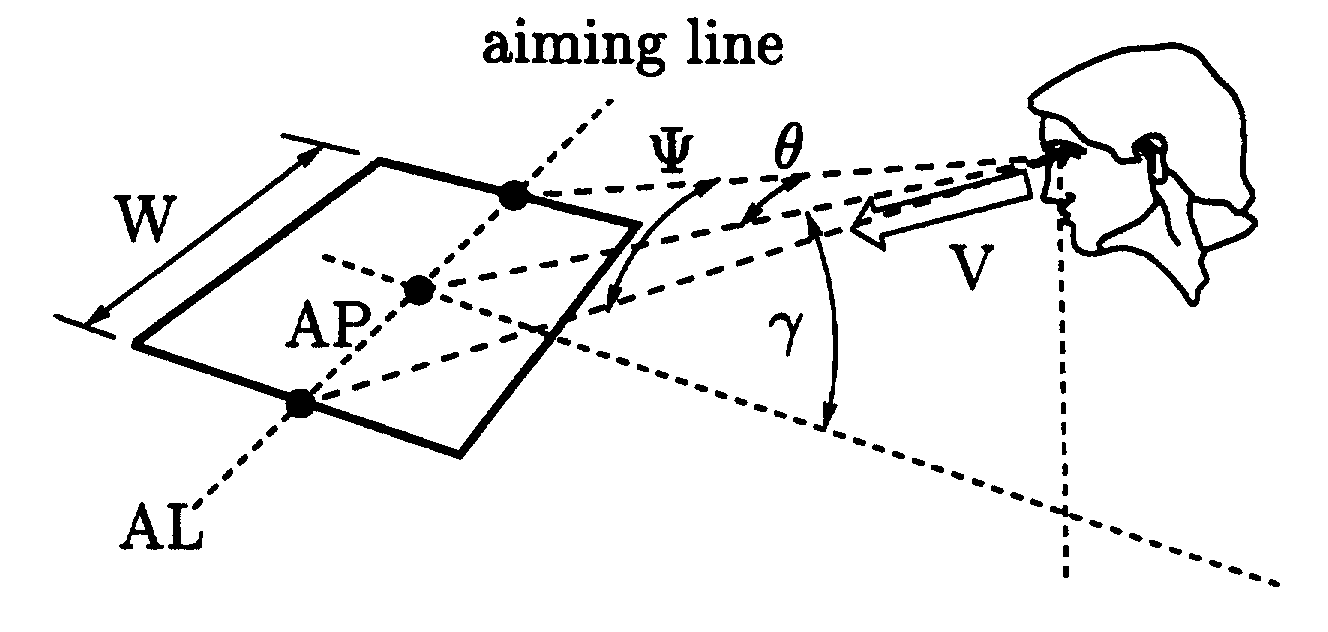
\includegraphics[width= \columnwidth]{visual_angle1.png} 
	\caption{\label{fig:visangle} Geometry of visual angle. [source \cite{Mulder2000}]}
\end{figure}

More precisely, the slope of each runway edge is related to the relative position and attitude of the aircraft. These relationships are given in \cite{Sasa2000}:

\begin{align}
\tilde{k_1} &= tan(atan(k_1) - \hat{\phi}) \\
\tilde{k_2} &= tan(atan(k_2) - \hat{\phi}) \\
\hat{h} &= \frac{\tilde{k_1} \tilde{k_2}}{\tilde{k_2} - \tilde{k_1}} \frac{cos(\hat{\theta})}{\cos(\hat{\psi})} B \label{eq:slope}
\end{align}

Where:
\begin{itemize}
\item $\hat{\phi}, \hat{\theta}, \hat{\psi}$ are the roll, pitch and heading estimates.
\item $k_1, k_1$ are the extracted runway edges
\item B is the runway width
\item $\hat{h}$ is the estimated altitude relative to the runway
\end{itemize}

Note that this slightly different than the cited paper. While \citeauthor{Sasa2000} use the horizon line to estimate the aircraft attitude, we are assuming that the roll, pitch and heading are available from inertial sensors on the phone.

\subsection{Runway Edge Extraction Pipeline}
We now describe how the runway edge extraction is performed. Note that part of this work is derived from the work of \cite{Naidu2011}.
\subsubsection*{\textbf{Cockpit Clutter Removal}}
\label{sec:pipeline:msk}
The first part of the pipeline is to differentiate between the portions of the image that constitute the out-of-the-window view, and those that constitute the interior view. The portions associated with the in-cockpit view are likely to be cluttered with information which will constitute noise when we try to detect the runway edges.

We experimented with two methods to remove cockpit clutter. In the first one, we averaged multiple frames together, and used subtracted the averaged image from each frame. In the second method, we simply used a brightness threshold to extract a mask, with the assumption that the cockpit is likely to be darker than the out-of-the-window view. In both cases, the mask was extracted in a pre-processing step, and used for all subsequent frames, i.e., the mask remained constant throughout the data processing.
A third alternative, which was not tested but is likely to be the simplest and more robust, is to allow the user on the phone interface to select which parts of the image are to be masked out.

\subsubsection*{\textbf{Image Dilation}}
Once the cockpit is removed, an image dilation operation as suggested by \cite{Naidu2011} is performed. We experimented with different stencils, and eventually settled on a $3\times3$ square stencil.
\subsubsection*{\textbf{Edge Detection and Area opening}}
We experimented with different edge detectors, but eventually settled on using the Sobel edge detector. The results of the edge detection were further processed by an expanded version of the background mask to remove the artifial edge of the mask itself. Additionally, an area opening operation to get rid of small regions was performed.
\subsubsection*{\textbf{Hough Transform}}
The detected edges are processed using a Hough transform for line detection. The range of angles that is being searched is restricted based on the previously detected runway edges. The initial range of angles requires an initialization, but a rough guess which can be deduced from coarse GPS altitude is sufficient.
\subsubsection*{\textbf{Line Scoring}} 
\label{sec:pipeline:score}
Each peak of the Hough transform is a candidate line in the original image. However, we are not interested in a single line, but rather in a pair of lines that represent the runway edges. Therefore, we take the top 20 peaks of the transform, and we form all possible $\binom{20}{2}$ pair combinations. Each pair is then scored and ranked. The score is designed to favor lines that exhibit the following properties:
\begin{itemize}
\item Assuming the pilot is approaching with a small side-slipe and along the runway centerline, we expect runway edges to be roughly symmetric to each other.
\item Likewise, we expect the pilot to be able to see the horizon during the approach, and therefore the lines should intersect within the image frame.
\end{itemize}
Additionally, we expect that between successive frames, the lines should not change too much from each other. Therefore, we keep track of a smoothed intersection point, and we score the line pairs based on their distance from this vanishing point.

\subsubsection*{\textbf{Altitude Extraction}}
The slopes from the best pair in the Hough transform are used to extract the estimated altitude per \cref{eq:slope}. Note that this requires knowing the aircraft attitude. There are two ways to determine the attitude. The first one is follow the method described in \cite{Sasa2000}, where the slope of the horizon line and the runway edges, as well as the position of the vanishing point, are used to infer the aircraft attitude (the horizon line can be extracted from the Hough transform). The second method is to assume that the aircraft attitude is provided by an inertial system. This is a reasonable assumption for this application since we are targetting an eventual implementation on a mobile device. 

\subsubsection*{\textbf{Kalman Filtering}}
\label{sec:pipeline:kalman}
Unfortunately, due to the various different noise sources, the identified lines and therefore the extracted visual altitude are likely to be noisy. However, if we think of the visual altitude as a noisy measurement in a stochastic process describing the aircraft altitude, we can combine it with other altitude measurements in a Kalman filter to smooth the predicted AGL. Some possible measurements that could be used include GPS altitude, GPS vertical velocity, and barometric pressure.
As mentioned previously, GPS on its own might not provide enough accuracy due to the large bias. Pressure altitude suffers from the same problem and can be laggy. The visual altitude on the other hand will have a fast time response and a small bias, but is likely to suffer from noise. We hypothesize that combining these two measurements would yield good results.


%Sec 4: Experiments — present your experimental results of the method you have implemented with plots, graphs, images and visualizations. Show numerical/quantitative and qualitative results. Show a performance analysis on the mobile device in term of efficiency, speed, memory and computational demands.
\section{Experimental results}
In this section, we describe our experimental setup and present examples of the different steps of the altitude extraction pipeline.
\subsection{Data collection}
A camera was installed inside of the cockpit of a Cessna 172, and multiple landings were performed. We decided to use Garmin Virb\texttrademark  \ camera to collect the data. We chose this camera because it was marketed as having GPS and attitude information as part of the metadata stored with the video. Unfortunately, it turned out that during our data collection, GPS measurements were only available at a low rate (1Hz), and we did not have any GPS velocities. Additionally, the attitude data was presented as accelerometer data which was very noisy due to vibrations in the airplane. This would be easily overcome if a reasonable attitude filter using gyro rates were to be used. Due to the lack of this data, we were forced to assume level flight.
We experimented with different camera settings, framerates, resolution, and camera locations. We eventually settled on wide field of view, 720p resolution, and 30 frames per second. A sample of the video frame sequence (in grayscale) is included in \cref{fig:raw}

\subsection{Pipeline Performance}
As mentioned in \cref{sec:pipeline:msk}, we experimented with two methods for masking the cockpit. We actually found that a combination of both methods worked best. I.e, we averaged the frames together, then applied the brightness threshold on the averaged to extract a mask which is subsequently used to remove the foreground (i.e. cockpit). The resulting masked image with dilation is shown in \cref{fig:msk}.

\begin{figure*}
\centering
\begin{subfigure}{\textwidth}
	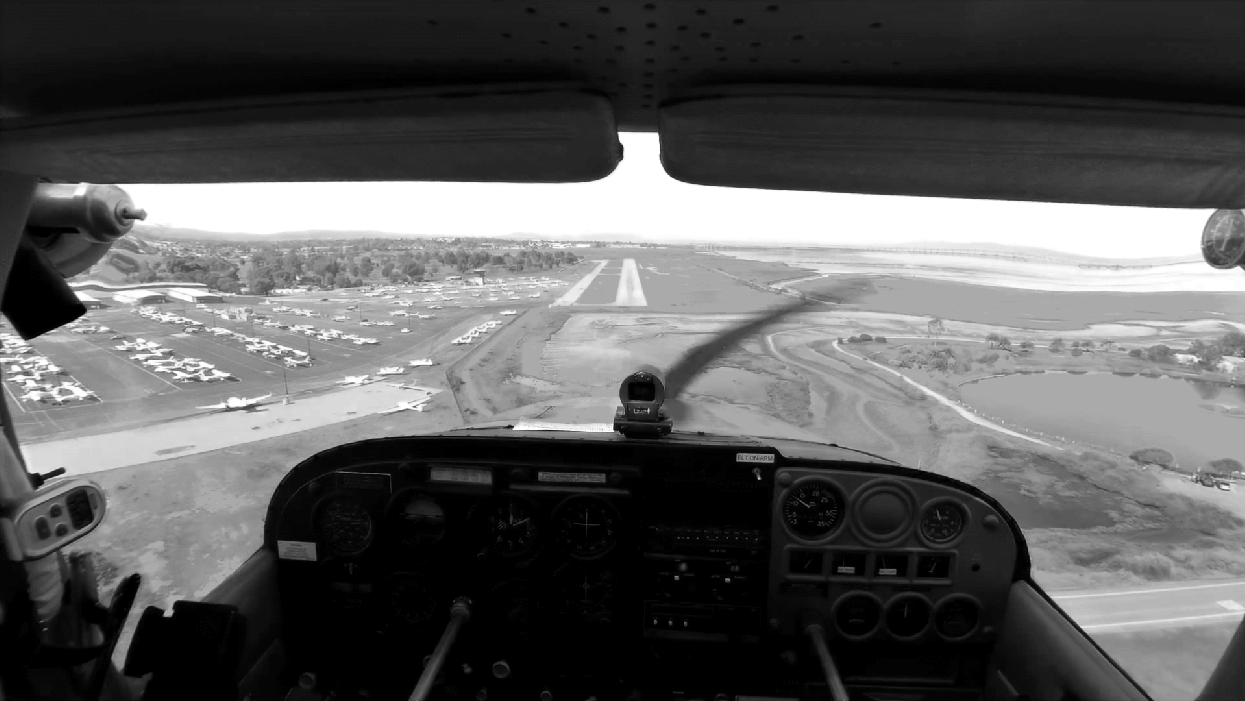
\includegraphics[width=\columnwidth]{raw.png} 
	\caption{\label{fig:raw} Raw grayscale frame}
\end{subfigure}
\begin{subfigure}{\textwidth}
    \centering
	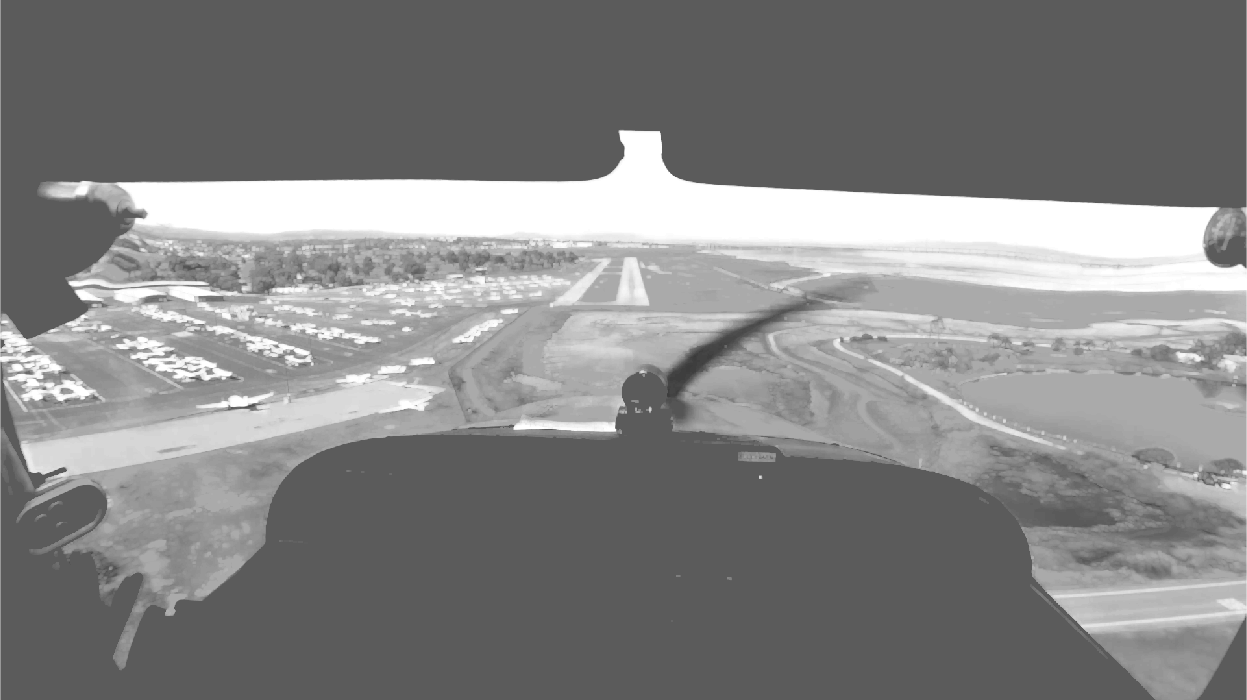
\includegraphics[width=\columnwidth]{mskdilated.png} 
	\caption{\label{fig:msk} Masked and Dilated frame}
\end{subfigure}
\caption{Runway Edge Detection Pipeline: Pre-Processing}
\end{figure*}


\begin{figure*}
\centering
\begin{subfigure}{0.85 \textwidth}
	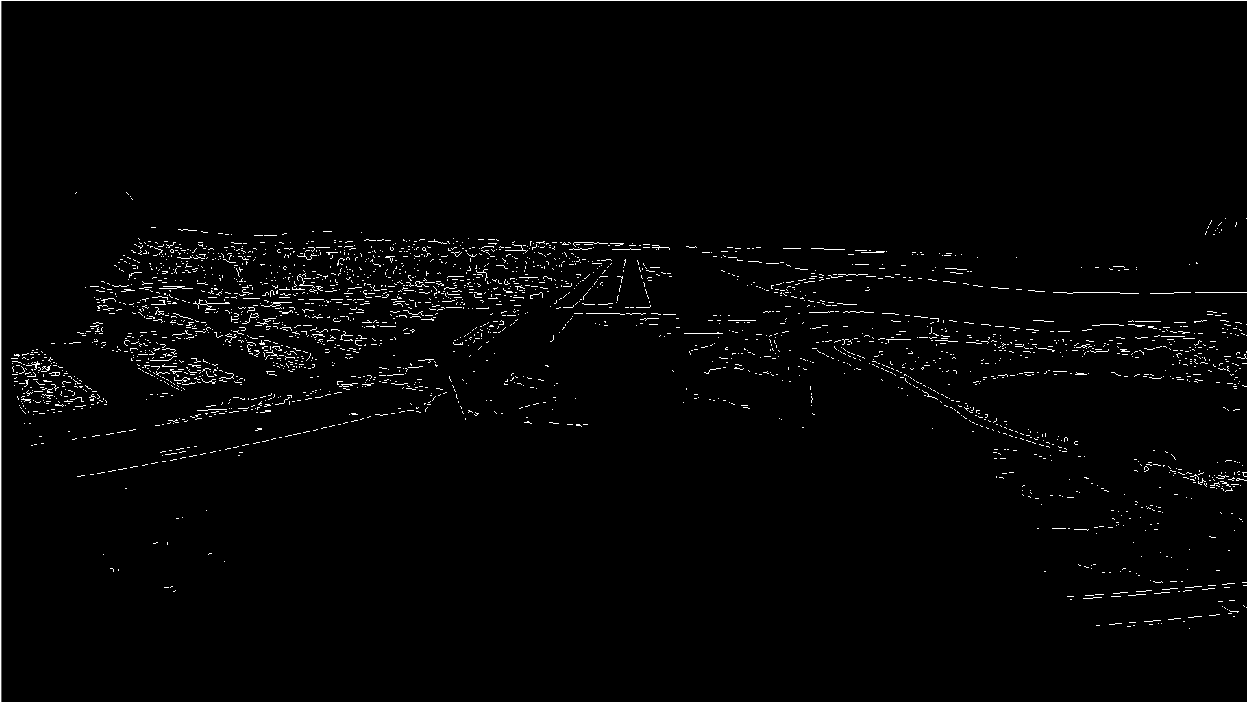
\includegraphics[width= \textwidth]{sobel.png} 
	\caption{\label{fig:sobel}  Sobel edge detection}
\end{subfigure}
\begin{subfigure}{0.85 \textwidth}
    \centering
	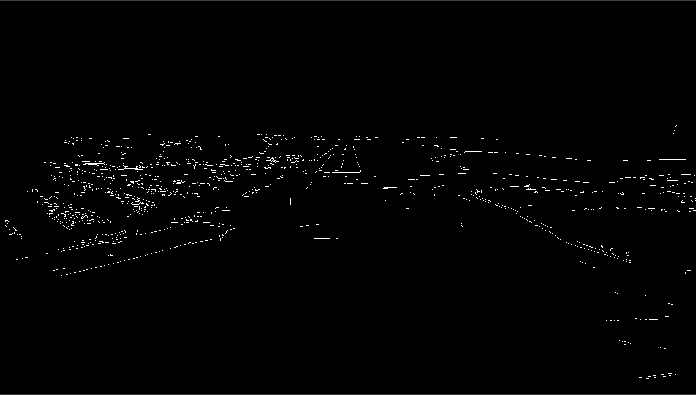
\includegraphics[width= \textwidth]{sobel_open.png} 
	\caption{\label{fig:sobelopen}Area Opening}
\end{subfigure}
\caption{Runway Edge Detection Pipeline: Edge detection}
\end{figure*}

A sample result of the edge detection is shown in \cref{fig:sobel}. Despite the area opening which removes some of the blobs as seen in \cref{fig:sobelopen}, many cluttered regions remain in the left portion of the image near the taxi area of the airport. We could further remove some of the blobs, but there is a trade-off to be made as a more aggressive area opening risks removing the runway edges themselves. 

\newpage

\begin{figure*}
\centering
\begin{subfigure}{\textwidth}
	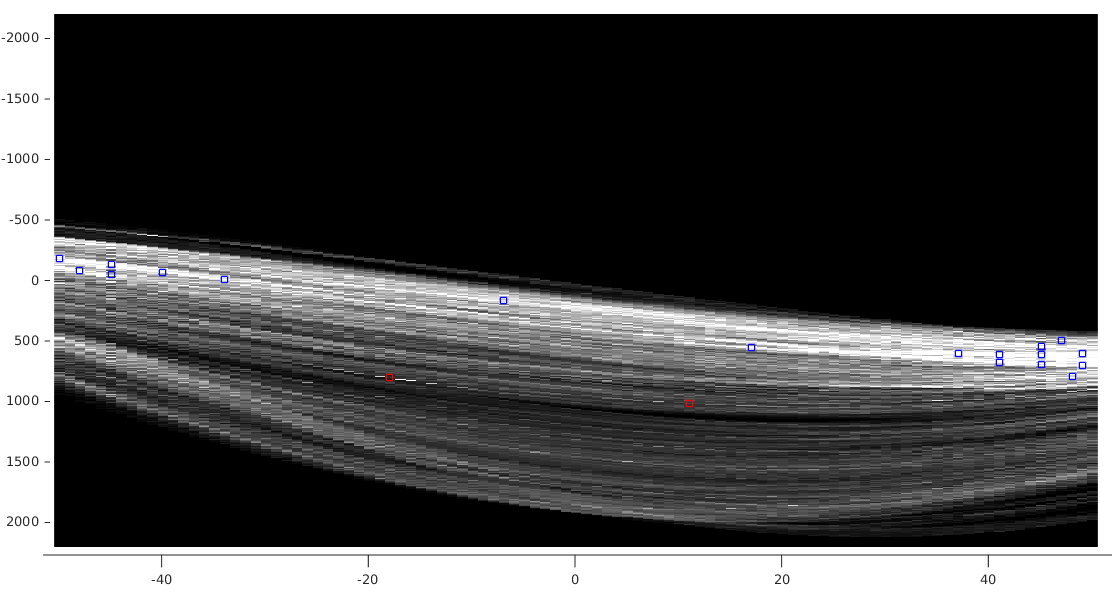
\includegraphics[width= \textwidth]{Hough.png} 
	\caption{\label{fig:Hough}  Hough Transform}
\end{subfigure}
\begin{subfigure}{\textwidth}
    \centering
	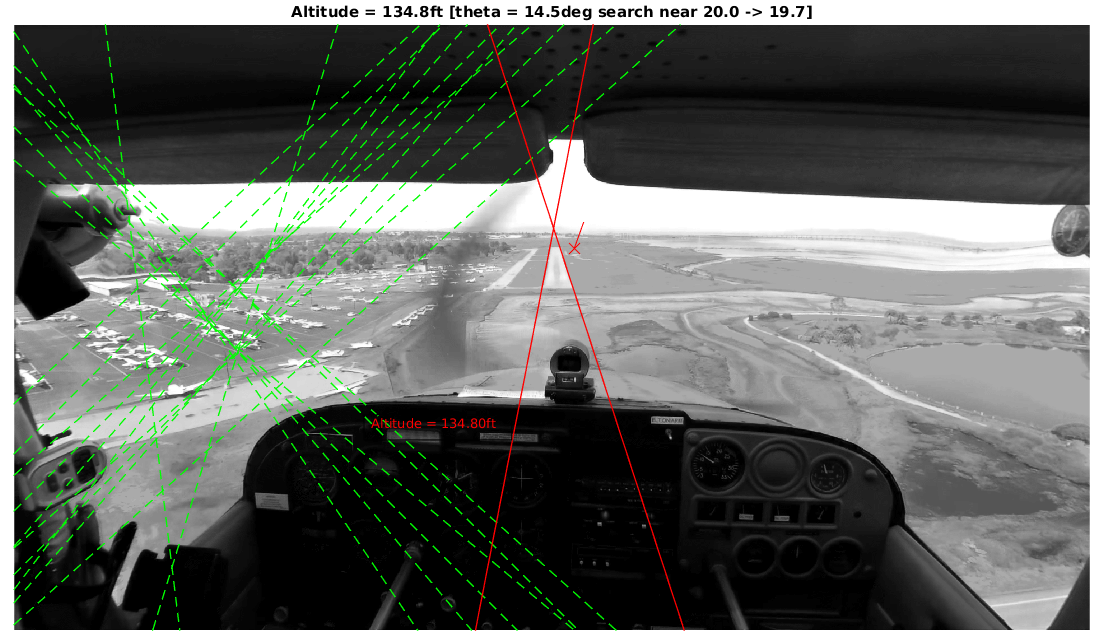
\includegraphics[width= \textwidth]{result.png} 
	\caption{\label{fig:final}  Detected Runway Edges}
\end{subfigure}
\caption{Runway Edge Detection Pipeline: Hough Transform}
\end{figure*}

A sample of the Hough transform for these images is shown in \cref{fig:Hough}. The top 20 lines are all identified in the Hough space in blue, and the top scoring pair is highlighted in red. All 20 lines are projected back into the 2D image in \cref{fig:final}.
\newpage

\begin{figure*}[ht]
\centering
	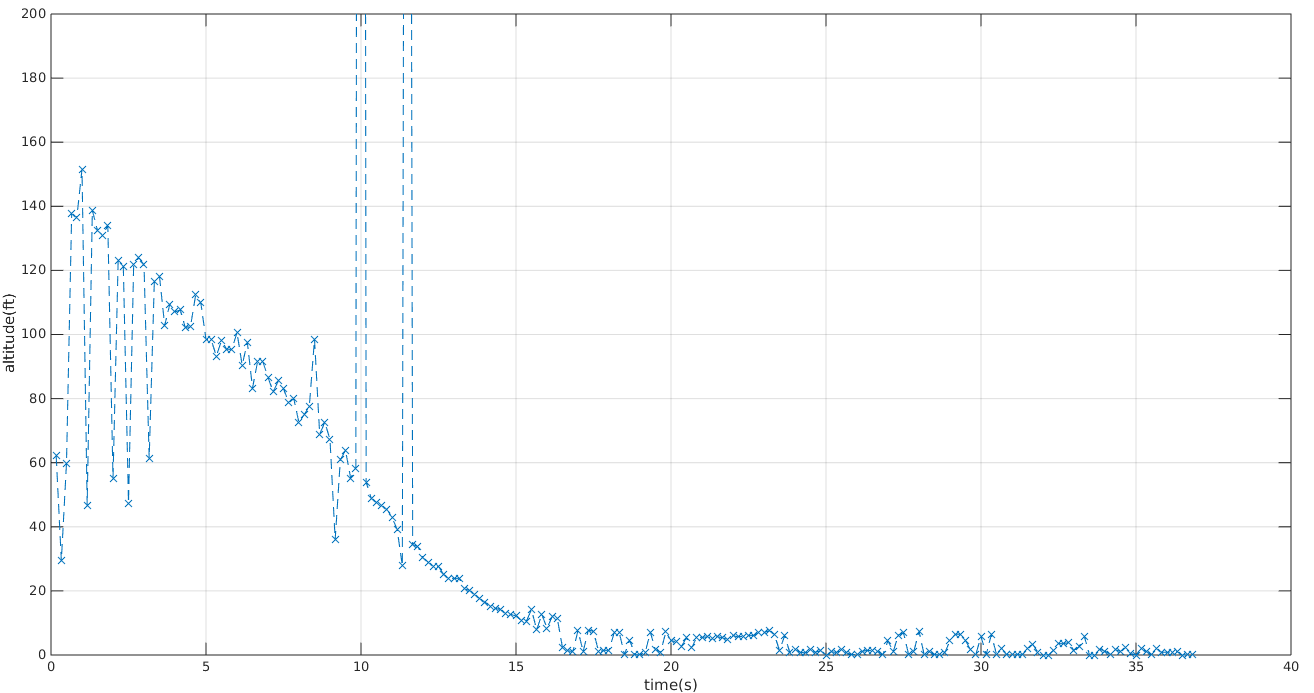
\includegraphics[width=  \textwidth]{alt.png} 
	\caption{\label{fig:alt}  Extracted Altitude from Video Sequence}
\end{figure*}


We notice in \cref{fig:final} that many of the false-positive lines go through the region with the blobs from the taxi area that were not removed by the area opening. But the top scoring pair (shown in red) correctly matches the runway edges. 

The slope of these two lines are then used to compute the above ground altitude using \cref{eq:slope}. The result is overlaid in text on \cref{fig:final}, where we can see that the extracted altitude ($\SI{134}{feet}$) matches the value displayed on the altimeter ($\SI{150}{feet}$) reasonably well (The airport is roughly at sea-level, so the altimeter is a good proxy for AGL).


The extracted altitude for a 30 seconds long portion is shown in \cref{fig:alt}. The results look reasonable. However, there are a few outliers in the results (some worse than others). We mentioned in \cref{sec:pipeline:kalman} that using a Kalman filter would smooth some of this noise and help reject outliers. Unfortunately, due to the problem with data collection in our first flights, combined with time constraints for this project, we were not able to collect data with other sensor values to experiment with the Kalman filtering.

Results of post-processing the video using the pipeline can be visualized at \url{http://youtu.be/QWjFQfFFzrY}

The Matlab source code for the pipeline described in this project is available at \url{http://github.com/zoohair/visioFlare}

%Sec 5: Conclusions — what's the take home message?
\section{Conclusions}
In this project, we implemented a runway edge detection pipeline using images captured from the cockpit view of an aircraft. We combined this pipeline with concepts from single view metrology to estimate the above ground altitude of a landing aircraft. Although the results were a bit noisy, the extracted altitude seemed reasonable.

We demonstrated the feasibility and soundness of the approach in this project, and we hope that this will get implemented on a phone in the future. The goal being that it can be used realtime in an aircraft to help student pilots improve their skills at the flare.

Unfortunately, due to problems gathering data and time constraints, we were not able to experiment with Kalman filtering to reduce some of the noise. However, we believe that outlier rejection should be possible based on innovation thresholding. Another way the Kalman filtering can be used in this framework is by tightly coupling it with the line-pair scoring part of the pipeline. Indeed, rather than scoring each pair based on the heuristic metrics we described in \cref{sec:pipeline:score}, we could treat each pair of lines as a potential measurement for the stochastic process. The innovation from each measurement can then be compared to the estimated covariance of the altitude, and measurements that have too large of an innovation can be rejected.

\newpage
%Sec 6: References.
\printbibliography


\end{document}